\documentclass[oneside]{scrbook}
\usepackage[colorlinks=true,linkcolor=blue,urlcolor=black,bookmarksopen=true]{hyperref}
\usepackage{bookmark}
\usepackage[dvipsnames]{xcolor}
\usepackage[round]{natbib}
\usepackage{amsfonts, amsthm, amsmath, amssymb, hyperref, cancel, wrapfig}
\usepackage{tikz, circuitikz, subfig, graphicx}
\usepackage{algpseudocode, algorithm}
\bibliographystyle{plainnat}

%%--CORRECTIONS--------------------------------------------------
\usepackage[switch, displaymath, mathlines]{lineno}
%\usepackage[allfiguresdraft]{draftfigure} % Disable pictures for fast rendering
\linenumbers{}
\counterwithin*{equation}{section}
\counterwithin*{equation}{subsection}

\newcommand\inlinetag{\stepcounter{equation}\ (\theequation)}


%%--MATH---------------------------------------------------------

% Custom Letters
\def\N{\ensuremath{\mathbb{N}}}
\def\Z{\ensuremath{\mathbb{Z}}}
\def\Q{\ensuremath{\mathbb{Q}}}
\def\R{\ensuremath{\mathbb{R}}}
\def\S{\ensuremath{\mathbb{S}}}

\usepackage{bbm,dsfont}
\def\1{\ensuremath{\mathds{1}}}
\def\E{\ensuremath{\mathbf{E}}\:}
\def\P{\ensuremath{\mathbf{P}}}
\def\A{\ensuremath{\mathcal{A}}}

% Custom text commands
\def\Var{\ensuremath{\mathbf{Var}}\,}
\def\Bi{\ensuremath{\mathrm{Bi}}}
\def\Be{\ensuremath{\mathrm{Be}}}

% Theorems and more
\newtheorem{theorem}{Theorem}[section]
\newtheorem{corollary}{Corollary}[theorem]
\newtheorem{lemma}[theorem]{Lemma}
\theoremstyle{remark}
\newtheorem*{remark}{Remark}

% Custom Commands
\newcommand{\angles}[1]{\ensuremath{\left\langle}#1\ensuremath{\right\rangle} }
\newcommand{\floor}[1]{\ensuremath{\left\lfloor}#1\ensuremath{\right\rfloor} }
\newcommand{\ceil}[1]{\ensuremath{\left\lceil}#1\ensuremath{\right\rceil} }

% \title{A Sample PhD Thesis}
% \author{A. N. Other}
% \date{July 2013}
% \titlehead{A Thesis submitted for the degree of Doctor of Philosophy}
% \publishers{School of Something\\University of Somewhere}

\begin{document}

% \maketitle

\frontmatter
\tableofcontents
\mainmatter{}

\chapter{Introduction}

\section{Basic inequalities and theorems}


%% --- Markov's inequality
\begin{theorem}[Markov's inequality]\label{markov}
  For a random variable $X$ with $\P\{X < 0\} = 0$ and $t>0$, we have
  \[ \P\{X \geq t\} \leq \frac{\E X}{t}.\]
  It follows that for a non-decreasing function $\varphi$ which only takes non-negative values,
  \[ \P\{X \geq t\} = \P\{\varphi(X) \geq \varphi(t)\} \leq \frac{\E\varphi(X)}{\varphi(t)}.\]
\end{theorem}

\vspace*{1em}

\begin{proof}
 In the first place, note that
 \[\arraycolsep=2pt
  \begin{array}{rrrll}
  X & = & X\cdot \1_{\{X \geq t\}} & + & X \cdot \1_{\{X < t\}}\\
    & \geq &t \cdot \1_{\{X \geq t\}} & + & 0,
 \end{array}\]
and thus,
\[ \E X \geq t \cdot \E \1_{\{X \geq t\}} = t \cdot \P\{X \geq t\}. \]
For the second statement, apply the same argument on the random variable $Y := \varphi(X)$ and the constant $s := \varphi(t)$.
\end{proof}
%% --------------------

\vspace*{2em}

%% --- Chebyshev's inequality
\begin{theorem}[Chebyshev's inequality]\label{chebyshev}
  For $t > 0$ and a random variable $X$ with mean $\mu = \E X$ and variance $\sigma^2 = \Var X$, then
  \[ \P\{|X-\mu| \geq t\} \leq \sigma^2 t^{-2}. \] 
\end{theorem}

\begin{proof}
  Applying Markov's inequality with $\varphi: x \mapsto x^2$ we obtain,
  \[ \P\{|X-\mu| \geq t \} = \P\{|X-\mu|^2 \geq t^2 \} \leq \frac{\E [{(X-\mu)}^2]}{t^2} = \sigma^2 t^{-2}.\] 
\end{proof}
%% --------------------

\vspace*{2em}

%% --- Jensen's inequality
\begin{theorem}[Jensen's inequality]\label{jensen}
  For any real valued random variable $X$ and convex function $\varphi$
  \[ \varphi(\E X) \leq \E \varphi(X). \] 
\end{theorem}

\begin{proof}[]
  
\end{proof}
%% --------------------


\vspace*{2em}

\section{Why bother?}

The concentration inequalities are used to obtain information on how a random variable is distributed at some specific places of its domain. In the most common scenarios, these inequalities will be used to quantify how concentrated a random variable at its tails, for example,

\[ \P\{|X-\mu| \geq t\} < f(t) << 1. \]

A concentration inequality is specially useful when this probability cannot be calculated at a low computational cost or estimated with high precision. The following  will illustrate a case where using concentration inequalities achieves the best results.

\subsection{Coin Tossing}

A coin tossing game is fair if the chances of winning are equal to the chances of losing. We can verify from a sample of $N$ games that the game is not rigged if the number of heads in the sample is not very distant from the average $N/2$. However, there's a chance that one may classify the coin as rigged, even when the coin is fair. By the \textit{Law of Large Numbers}, we know that the larger the sample, the less likely it is to obtain a false positive. But let's ask ourselves how fast this probability converges to 0.

\vspace*{1em}

Let $S_N \sim \Bi(N,1/2)$ denote the number of heads in a fair coin tossing game. Then,
\[ \mu = \E S_N = \frac{N}{2}, \hspace*{2em} \sigma^2 = \Var S_N = \frac{N}{4}. \] 
For a fixed $\varepsilon > 0$, we may classify a coin tossing game as rigged if, after $N$ trials, the ratio of heads vs tails in the sample is greater than $[1+\varepsilon:1-\varepsilon]$, or similarly,
\[ S_N \geq \mu +  \frac{\varepsilon}{2} N = \frac{1+\varepsilon}{2} N. \]

Using the Chebyshev inequality~\ref{chebyshev}, we assert that

\[ \P\left\{S_N \geq \mu +  \frac{\varepsilon}{2} N\right\} \leq 
\P\left\{|S_N-\mu| \geq  \frac{\varepsilon}{2} N\right\} \leq \sigma^2 \frac{4}{\varepsilon^2 N^2} = \frac{1}{\varepsilon^2 N}.\] 

Therefore, the probability of bad events tends to 0 at least linearly with the number of games.

\subsection{Central Limit Theorem}

The proof of the following theorems can be found in (ref)

%% --- Central Limit Theorem
\begin{theorem}\label{centrallimit}
    Let $X_i$ be a i.i.d.~sample. Let $S_N = \sum_{i = 1}^N X_i$, with mean $\mu = \E S_N$ and variance $\sigma^2 = \Var S_N$. If  
    \[ Z_N =  \frac{S_N - N\cdot \E X_i}{\sqrt{N \cdot \Var X_i}} =  \frac{S_N - \mu}{\sqrt{N}\sigma},\] 
    then,
    \[ Z_N \to Z \sim \mathcal{N}(0,1),\hbox{ in distribution.} \] 

    \hfill $\square$
\end{theorem}
%% --------------------

\vspace*{2em}

%% --- Central Limit Theorem
\begin{theorem}[Tails of the Normal Distribution]\label{normaltails}
    Let $Z\sim \mathcal{N}(0,1)$, for $t>0$ we have
    \[ \left( \frac{1}{t}-\frac{1}{t^3}\right) \frac{1}{\sqrt{2\pi}} \exp\left(\frac{-t^2}{2}\right) \leq \P\{Z \geq t\} \leq \frac{1}{t}\;\frac{1}{\sqrt{2\pi}} \exp\left(\frac{-t^2}{2}\right). \]

    \hfill $\square$
\end{theorem}
%% --------------------

With that in mind, we might naively assume that better bounds can be obtained by using the previous theorem. For a large enough $N$ we can say that for the coin tossing,
\[ Z_N = \frac{S_N- N/2}{\sqrt{N/4}} \] 
\[ \implies \P \left\{S_N \geq \frac{1+\varepsilon}{2} N \right\} = \P\left\{Z_N \geq \varepsilon \sqrt{N} \right\} \sim \P\left\{Z \geq \varepsilon \sqrt{N} \right\}.\]
However, this raises the question of whether we can draw the following conclusion from Theorem~\ref{normaltails}:
\[ \P \left\{S_N \geq \frac{1+\varepsilon}{2} N \right\} \leq \frac{1}{\varepsilon \sqrt{N}}\;\frac{1}{\sqrt{2\pi}} \exp\left(\frac{-\varepsilon^2 \cdot N}{2}\right). \]
Unfortunately, the answer is no. The following theorem will show why.


%% --- Berry-Essen CLT
\begin{theorem}[Convergence Rate for Central Limit Theorem]\label{berryessen}
  For $Z_N$, $Z$ in Theorem~\ref{centrallimit}, we have:
  \[ \left|\P\{Z_N \geq t\} - \P\{Z \geq t\}\right| = O(\tfrac{1}{\sqrt{N}}). \]
  \hfill $\square$
\end{theorem}
%% --------------------

Since the approximation error is greater than the bound, the previous results cannot be taken into account.

In the context of coin tossing, this may not matter at all because the linear bound obtained using Chebyshev's inequality indicates that the probability of wrongly classifying a fair coin as a rigged coin converges at least linearly to zero. Even the Central Limit Theorem shows in a less precise way this convergence. However, for some specific problems in statistics, these basic tools are not precise enough to solve them. In the following chapters, we will show some examples were better crafted strategies are needed in order to get bounds to the tails of the random variables.

\chapter{Exponential Inequalities}

Even if we are satisfied with the linear convergence rate provided by Chebyshev's inequality or the improvement of one sided tails given by Cantelli's inequality, there is a simple but powerful modification we can make to Markov's inequality that will greatly improve both bounds. The following result will provide the main idea from which most of the exponential inequalities are derived.

%% --- MGF Inequality
\begin{theorem}[MGF inequality]\label{mgf}
  Let $X_i$ be a finite sequence of independent random variables and let $S_N := \sum_{i = 1}^N a_i X_i$. Let $\lambda > 0$. The following inequality holds,
  \[ \P\left\{  S_N \geq t\right\} \leq e^{-\lambda t}\cdot \prod_{i = 1}^N \E e^{\lambda a_i X_i}. \] 

\end{theorem}

\begin{proof}
  Let $\lambda > 0$, using Markov's inequality (Theorem~\ref{markov}) we assert that since $x\mapsto e^{\lambda x}$ is a non-decreasing function,
  \[ \P\left\{  S_N \geq t\right\} = \P\left\{  e^{\lambda S_N} \geq e^{\lambda t}\right\} \leq e^{-\lambda t} \cdot \E \exp\left( \lambda \sum_{i = 1}^N a_i X_i \right). \]
  Since $X_i$ are independent, the MGF of $S_N$ is the product of MGFs of each $X_i$:
  \[\E \exp\left( \lambda \sum_{i = 1}^N a_i X_i \right) = \prod_{i = 1}^N \E e^{\lambda a_i X_i} \] 
  \[ \implies \P\left\{  S_N \geq t\right\} \leq e^{-\lambda t}\cdot \prod_{i = 1}^N \E e^{\lambda a_i X_i}. \]
\end{proof}
%% --------------------

The following two theorems are examples on how we can obtain even tighter bounds than the ones we've already studied. In particular, these theorems can be obtained from the previous theorem and are considered, by some authors, as corollaries of the previous result.

%% --- Chernoff's inequality
\begin{theorem}[Chernoff's inequality]\label{chernoff:bernoulli}
  Let $X_i \sim \Be(p_i)$ be independent random variables. Define $S_N = \sum_{i = 1}^{N} X_i$ and let $\mu = \E S_N$. Then, for $t > \mu$, we have
  
  \[ \P\left\{  S_N \geq t\right\} \leq  {\left(\frac{\mu}{t}\right)}^t e^{-\mu+t} .\] 
\end{theorem}

\begin{proof}
  In the first place, use Theorem~\ref{mgf} to assert that for a $\lambda > 0$ that
  \[\P\left\{  S_N \geq t\right\} \leq e^{-\lambda t}\cdot \prod_{i = 1}^N \E e^{\lambda X_i}.\] 
  Now it is left to bound every $X_i$ individually. Using the inequality $1+x \leq e^x$ we obtain
  \[ \E e^{\lambda X_i} = e^{\lambda}p_i + (1-p_i) = 1 + (e^{\lambda}-1)p_i  \leq \exp(e^{\lambda}-1)e^{p_i}.\]
  Finally, we plug this inequality on the equation to conclude that
  \[e^{-\lambda t}\cdot \prod_{i = 1}^N \E e^{\lambda X_i} \leq e^{-\lambda t}\cdot \prod_{i = 1}^N \exp((e^{\lambda}-1) p_i) = e^{-\lambda t} \exp((e^{\lambda}-1) \mu). \]
  By using the substitution $\lambda = \ln (t/\mu)$ we obtain the desired result,
  \[ \P\left\{  S_N \geq t\right\} \leq {\left(\frac{\mu}{t}\right)}^t \exp{\left(\frac{\mu t}{\mu}-\mu\right)} = {\left(\frac{\mu}{t}\right)}^t e^{-\mu+t}. \]
\end{proof}
%% --------------------

Another exponential inequality that is derived using a similar technique is Hoeffding's inequality:

%% --- Hoeffding's inequality
\begin{theorem}[Hoeffding's inequality]\label{hoeffding:bounded}
  Let $X_1, \ldots, X_N$ be independent random variables, such that $X_i \in [a_i,b_i]$ for every $i = 1,\ldots,N$. Define $S_N = \sum_{i = 1}^{N} X_i$ and let $\mu = \E S_N$. Then, for every $t > 0$, we have
  \[ \P\left\{  S_N \geq \mu + t\right\} \leq \exp\left( \frac{-2t^2}{\sum{( a_i - b_i )}^2}\right). \]
\end{theorem}

\begin{proof}
  Since, for $\lambda > 0$, $x \mapsto e^{\lambda x}$ is a convex function, it follows that, for any bounded random variable $X \in [a,b]$:
  \[ e^{\lambda X} \leq \frac{e^{\lambda a}(b-X)}{b-a} + \frac{e^{\lambda b}(X-a)}{b-a},\hspace*{1em} a \leq b. \]
  Then, take expectations on both sides of the equation to obtain:
  \[ \E e^{\lambda X} \leq \frac{(b-\E X) \cdot e^{\lambda a}}{b-a} + \frac{(\E X -a) \cdot e^{\lambda b}}{b-a}. \]
  To simplify the expression, let $\alpha = (\E X -a)/(b-a)$, $\beta = (b-\E X)/(b-a)$ and $u = \lambda (b-a)$. Since $a < \E X < b$, it follows that $\alpha$ and $\beta$ are positive. Also, note that,
  \[ \alpha + \beta = \frac{\E X-a}{b-a} + \frac{b-\E X}{b-a} = \frac{b-a}{b-a} = 1. \] 
  Now,
  \[ \ln \E e^{\lambda X} \leq \ln (\beta e^{-\alpha u} + \alpha e^{\beta u}) = -\alpha u + \ln(\beta + \alpha e^{u}). \] 
  This function is differentiable with respect to $u$.
  \[\everymath{\displaystyle}\arraycolsep=1.8pt\def\arraystretch{1.8}
    \begin{array}{rcl}
    L(u) & = & -\alpha u + \ln(\beta + \alpha e^{u}),\\
    L'(u) & = & -\alpha + \frac{\alpha}{\alpha + \beta e^{-u}},\\
    L''(u) & = & \frac{\alpha}{\alpha + \beta e^{-u}} \cdot \frac{\beta e^{-u}}{\alpha + \beta e^{-u}}.
  \end{array} \]
  Note that if $x = \frac{\alpha}{\alpha + \beta e^{-u}} \leq 1$, then $L''(u) = x(1-x) \leq \frac{1}{4}$. Remember that $\alpha + \beta = 1$. Now, by expanding the Taylor series we obtain,
  \begin{equation}
    \tag{$\star$} \everymath{\displaystyle}\arraycolsep=1.8pt\def\arraystretch{2}
  \begin{array}{rcl}
    L(u) & = & L(0) + uL'(0) + \frac{1}{2} u^2 L''(u)\\
    & = &\ln(\beta + \alpha) + u \left(-\alpha + \frac{\alpha}{\alpha + \beta}\right) + \frac{1}{2} u^2 L''(u) \\
    & = & \frac{1}{2} u^2 L''(u)\\
    &\leq & \frac{1}{8}\lambda^2 {(b-a)}^2.
  \end{array}
  \end{equation}

  Finally, use the inequality from Theorem~\ref{mgf} to conclude that
  \[\everymath{\displaystyle}\arraycolsep=1.8pt\def\arraystretch{2}
    \begin{array}{rcl}
      \P\{S_N-\mu \geq t\} & \leq & e^{-\lambda t} \prod_{i = 1}^N \E e^{\lambda X_i} \\
      &\leq^{(\star)} & e^{-\lambda t} \exp\left(\frac{1}{8}\lambda^2 \sum_{i = 1}^{N} {(b_i-a_i)}^2\right).
    \end{array}\] 

  Use the substitution $\lambda = 4t {\left(\sum_{i=1}^N{(b_i-a_i)}^2\right)}^{-1}$ to get the desired result.

\end{proof}
%% --------------------



%% --- Hoeffding's inequality (Bernoulli)
\begin{corollary}\label{hoeffding:bernoulli}
  Let $X_1,\ldots, X_N$ be independent random Bernoulli variables such that $X_i \sim \Be(p_i)$, then
  \[ \P\left\{ \sum_{i = 1}^N (X_i - p_i) \geq t\right\} \leq \exp\left( \frac{-2t^2}{N}\right). \] 
\end{corollary}

\begin{proof}[]

\end{proof}
%% --------------------

Returning to the coin tossing problem, we can now make a stronger assertion of the rate of convergence of a false negative classification using Hoeffding inequality:
\[\P \left\{S_N- \frac{N}{2} \geq \frac{\varepsilon}{2} N \right\} \leq \exp\left( - \varepsilon^2 N \right). \] 

% However, this raises the question of which of the previous inequalities is better for a given problem. In the previous case, we chose Hoeffding's inequality, but when dealing with any specific problem, one needs to determine the criteria for deciding whether it's more appropriate to use Chernoff, Hoeffding, or any other inequality. In the following section, we will try to identify situations where one of these inequalities is more suitable than the other.



\section{Uniform Law of Large Numbers}
For any probability measure $P$ on the real line and $t \in \R$, define $P_n$ as the empirical probability measure obtained from an independent sample $X_1, \ldots, X_n$ of $P$, that is:
\[ P_n(t) = P_n(-\infty, t) = n^{-1} \cdot \sum_{i = 1}^n \1_{\{ X_i \leq t\}}.\]

From the law of large numbers we know that for a fixed $t$, $P_n(t)$ converges to $P(t)$ with probability 1. However we can formulate a stronger statement on this convergence. The first application of concentration inequalities we are going to explore is the uniform law of large numbers, which states the following:

\begin{theorem}[Glivenko-Cantelli Theorem]\label{glivenko-cantelli}
  For $P,\; P_n$ and $t \in \R$,
  \[ \|P_n - P\| = \sup_{t\in \Q} \left|P_n(t) - P(t)\right| \overset{p}{\longrightarrow} 0.\]  
\end{theorem} 

\begin{proof}
  The proof, adapted from~\cite{pollard1984convergence}, consists of 5 steps. At first instance, the author clarifies that we can impose the condition $t\in \Q$ to avoid problems with measurability. The author later proves that the theorem is true if $t$ is allowed to vary in $\R$, but for practical purposes, we will only prove it for rationals. Another remark the author makes is that this result from the real line can be later generalized for some classes of ``polynomial discrimination'', and we will cover more about this in the final section.

  \subsubsection*{First Symmetrization}
  In the first place, define $P_n'$ as the empirical measure obtained from an independent but identical sample $X_1',\ldots, X_n'$ of $P$. Note that for any fixed $t$, $P_n(t)$ and $P_n'(t)$ are random variables derived from their respective samples which satisfy that
  \[ \E P_n(t) = \E P_n'(t) = P(t). \] 
  We will bound the concentration of $\|P_n- P_n'\|$ first, which will later result in a bound for $\|P_n - P\|$ at the end of the following lemma.

  \vspace*{1em}

  For now, fix a value for $\varepsilon > 0$, and keep in mind that $Z = P_n - P$, $Z' = P_n' - P$, $\alpha = \frac{1}{2}\varepsilon$ and $\beta = \frac{1}{2}$. Also, for this case define $\AA = \{(-\infty, t) : t\in \R\}$

  \begin{lemma}\label{gc:l1}
    Let ${\{Z(A)\}}_{A\in \AA}$ and ${\{Z'(A)\}}_{A\in \AA}$ be independent and identical functions defined over the same collection of sets $\AA$. Also, assume that there exist $\alpha, \beta > 0$ such that
    \[ \P\left\{|Z(A)| \leq \alpha \right\} \geq \beta, \hspace*{1em} \forall A \in \AA \]
    It follows that, for any $\varepsilon > 0$,
    \[  \P\left\{\sup_{A\in \AA} |Z(A)| > \varepsilon \right\} \leq \beta^{-1} \P\left\{\sup_{A\in \AA} |Z(A)-Z'(A)| > \varepsilon - \alpha \right\}. \]     
  \end{lemma}

  \begin{proof}
    Fix an index $B$ in the set $T_\varepsilon = \{ A \in \AA \;:\; |Z(A)| > \varepsilon\}$.
    it follows from the independence of $Z$ and $Z'$ that,

    \[ \beta \cdot \P \{ T_\varepsilon \neq \emptyset\} \leq \P \{ T_\varepsilon \neq \emptyset \text{ and }  |Z'(B)|\leq \alpha \} \] 

    Now, if $T_\varepsilon \neq \emptyset \text{ and }  |Z'(B)|\leq \alpha  $, then $|Z'(B)| \leq \alpha\text{ and } |Z(B)| > \varepsilon$. Thus, since $\sup_{A\in \AA} |Z(A)| > \varepsilon$ implies $T_\varepsilon \neq \emptyset$, it follows that

    \[\everymath{\displaystyle}\arraycolsep=1.8pt\def\arraystretch{1.8}
    \begin{array}{rcl}
      \beta \cdot \P\left\{\sup_{A\in \AA} |Z(A)| > \varepsilon \right\} & \leq & \P\{|Z'(B)| \leq \alpha\text{ and } |Z(B)| > \varepsilon\}\\
       & \leq & \P\{ |Z(B) - Z'(B)| > \varepsilon - \alpha \}\\
        & \leq & \P\left\{\sup_{A\in \AA} |Z(A)-Z'(A)| > \varepsilon - \alpha \right\}.
    \end{array} \] 
  \end{proof}
  Using Chevyshev's inequality (\ref{chebyshev}) we know that the hypothesis is satisfied for the values of $\alpha$ and $\beta$ we chose:
  \[\forall t\in \R: \P\left\{ |Z'(t)| \leq \alpha \right\} = \P\{|P_n(t) - P(t)| \leq \varepsilon\} \geq \frac{1}{2} = \beta,\hspace*{1em} \text{if $n \geq 8\varepsilon^{-2}$}.\]
  Therefore, using the previous lemma, we conclude that
  \begin{equation}
    \label{gc:1} 
    \P\{\|P_n-P\| > \varepsilon\} \leq 2 \P\{\|P_n-P_n'\| > \tfrac{1}{2} \varepsilon\},\hspace*{1em} \text{if $n \geq 8\varepsilon^{-2}$}.
  \end{equation}

  \vspace*{1em}

  \subsubsection*{Second Symmetrization}
  The following trick will allow us to stop considering all of the $2n$ data points from the previous symmetrization, and will help us to create a simpler random variable. We will initially prove the trick for unidimensional random variables, but in chapter 4, we will generalize this proof for any kind of set on $\R^n$.

  \begin{lemma}\label{gc:l2}
    Let $\sigma_1, \ldots, \sigma_n$ be Rademacher i.i.d.~random variables, that is $\P\{\sigma_i = 1\} = \P\{\sigma_i = -1\} = 1/2$, and they are independent from $X_i$ and $X_i'$. Let $Y_i = \1_{\{ X_i' \in A\}} - \1_{\{ X_i \in A\}}$, and note that,
    \[ \P\{Y_i = x\} = \P\{\sigma_i Y_i = x\},\hspace*{1em} x \in \{-1,0,1\}. \] 
  \end{lemma}

  \begin{proof} In the first place, since $X_i$ and $X'_i$ are two independent and identical copies of the same distribution, the following equality holds: 

    \[ \begin{array}{rcl}
      \P\{Y_i = 1\} & = & \P\{X_i \in A\} \P\{X'_i \not\in A\}\\
      & = &  \P\{X'_i \in A\} \P\{X_i \not\in A\}\\
      & = & \P\{Y_i = -1\}.
    \end{array} \]
  On the other hand, since $\sigma_i$ is also independent of $Y_i$, it follows that
  \[ \everymath{\displaystyle}\arraycolsep=1.8pt\def\arraystretch{1.8}
  \begin{array}{rcl}
    \P\{\sigma_i Y_i = 1\} & = & \P\{Y_i = 1, \sigma_i = 1\} + \P\{Y_i = -1, \sigma_i = -1\}\\
    & = & \P\{Y_i = 1\} \P\{\sigma_i = 1\} + \P\{Y_i = -1\} \P\{\sigma_i = 1\}\\
    & = & \frac{1}{2} \P\{Y_i = 1\} + \frac{1}{2} \P\{Y_i = 1\}\\
    & = & \P\{Y_i = 1\} = \P\{Y_i = -1\} = \P\{\sigma_i Y_i = -1\}.
  \end{array}
    \]
    Thus,
    \[  \P\{\sigma_i Y_i = \pm 1\} = \P\{Y_i = \pm 1\},\hspace*{1em}  \P\{\sigma_i Y_i = 0\} = \P\{ Y_i = 0\}. \] 
  \end{proof}
  
  It follows that since $P_n - P_n' = n^{-1} \sum_{i \leq n} Y_i$,
  \begin{equation}
    \label{gc:2} 
    \everymath{\displaystyle}\arraycolsep=1.8pt\def\arraystretch{3}
  \begin{array}{rcl}
    \P\{\|P_n - P_n'\| > \tfrac{1}{2}\varepsilon\} & = & \P\left\{\sup_{t\in \Q} \left|n^{-1}\sum_{i = 1}^n \sigma_i Y_i\right| >\tfrac{1}{2}\varepsilon \right\}\\
    & \leq & \P\left\{\sup_{t\in \Q} \left|n^{-1}\sum_{i = 1}^n \sigma_i\1_{\{ X_i < t\}}\right| >\tfrac{1}{4}\varepsilon \right\}\\
    & & + \P\left\{\sup_{t\in \Q} \left|n^{-1}\sum_{i = 1}^n \sigma_i\1_{\{ X_i' < t\}}\right| >\tfrac{1}{4}\varepsilon \right\}
  \end{array}
  \end{equation}
  \[ = 2\P\{\|P_n^\circ\| > \tfrac{1}{4} \varepsilon\}.  \] 
  where $P_n^\circ = n^{-1}\sum_{i\leq n} \sigma_i \1_{\{ X_i < t\}}$. Then, from equations $\ref{gc:1},\;\ref{gc:2}$ we conclude that for $n \geq 8\varepsilon^{-2}$,
  \[ \P\{\|P_n-P\| > \varepsilon\} \leq 4 \P\{\|P_n^\circ\|> \tfrac{1}{4}\varepsilon\}.\]

  \vspace*{1em}

  \subsubsection*{Maximal Inequality}

  \[\begin{tikzcd}
    {-\infty} & {X_{(1)}} & {X_{(2)}} & {X_{(3)}} & \cdots & {X_{(n)}} & \infty
    \arrow["{t_1}", no head, from=1-2, to=1-3]% chktex 18
    \arrow["{t_2}", no head, from=1-3, to=1-4]% chktex 18
    \arrow["{t_3}", no head, from=1-4, to=1-5]% chktex 18
    \arrow["{t_{n-1}}", no head, from=1-5, to=1-6]% chktex 18
    \arrow["{t_0}"', from=1-2, to=1-1]% chktex 18
    \arrow["{t_n}", from=1-6, to=1-7]% chktex 18
  \end{tikzcd}\]

  For any given sample $X = X_1, \ldots, X_n$, define $X_{(j)}$ as the $j$-th observation when we order the observations, and fix $t_j \in (X_{(j)}, X_{(j+1)}]$ for every $j\leq n$ as the picture above shows. Note that if $t \in (X_{(j)}, X_{(j+1)}]$, then $P_n^\circ (t) = P_n^\circ (t_j)$ because:  % chktex 9

  \[ \everymath{\displaystyle}\arraycolsep=1.8pt\def\arraystretch{1.8}
  \begin{array}{rclcl}
    P_n^\circ (t) & = & n^{-1}\sum_{i = 1}^n \sigma_i\1_{\{ X_i < t\}}, & & \hfill t \in (X_{(j)}, X_{(j+1)}] \\ % chktex 9
    & = & n^{-1}\sum_{i = j+1}^{n} \sigma_i\1_{\{ X_{(i)} < t\}} & + & n^{-1} \sum_{i = 1}^{j} \sigma_i \1_{\{ X_{(i)} < t\}}\\
    & = & n^{-1}\sum_{i = j+1}^{n} \sigma_i \cdot 1 & + &  \hfill0\hfill\\
    & = & P_n^\circ (t_j).
  \end{array}
  \]

  It follows that for some $k$, $\|P_n^\circ\| = |P_n^\circ (t_k)|$, and thus,
   \begin{equation} \label{gc:3}
    \everymath{\displaystyle}\arraycolsep=1.4pt\def\arraystretch{1.5}
    \begin{array}{rcl}
      \P\{ \|P_n^\circ\| > \tfrac{1}{4} \varepsilon \;|\; X \} & \leq & \sum_{j = 0}^n \max_j \P\{ |P_n^\circ(t_j)| > \tfrac{1}{4} \varepsilon \;|\; X \}\\
      & \leq & (n+1) \cdot \P\{ |P_n^\circ(t_k)| > \tfrac{1}{4} \varepsilon \;|\; X \} .
    \end{array} 
  \end{equation}
  \vspace*{1em}

  \subsubsection*{Exponential Bounds}

  Since for any given sample, $\sigma \1_{X_i < t} \in [-1,1]$, we can use Hoeffding's Inequality~\ref{hoeffding:bounded} to obtain the following inequality
  \[ \P \{ |P_n^\circ(A)| > \tfrac{1}{4} \varepsilon \} \leq 2 \exp\left( \frac{-2{(n\varepsilon/4)}^2}{4n}\right) = 2e^{-n\varepsilon^2/32}, \hspace*{1em} \forall A \in \AA.\]
  We use equation $\ref{gc:3}$ to conclude
  \begin{equation} \label{gc:4}
    \P\{ \|P_n^\circ\| > \tfrac{1}{4} \varepsilon \;|\; X\} \leq 2(n+1) e^{-n\varepsilon^2/32}.
  \end{equation} 

  \vspace*{1em}

  \subsubsection*{Integration}

  Finally, applying the formula $P\{A\} = \E_X[\P\{A | X\}]$, we conclude that

  \begin{equation}
    \label{gc:5}\begin{array}{rcl}
      \P \{\|P_n-P\| > \varepsilon\} & = & \E [\P \{\|P_n-P\| > \varepsilon \;|\; X\}]\\
      & \leq & \E [8(n+1) e^{-n\varepsilon^2/32}]\\
      & = & 8(n+1) e^{-n\varepsilon^2/32}.
    \end{array} 
  \end{equation}

  The Borel-Cantelli Lemma states that if the probability of a sequence of events is summable, that is \(\sum_{n = 1}^\infty \P\{E_n\} < \infty\), then
  \begin{equation}\label{borel-cantelli}
    \limsup_n \P(E_n) = \P \left\{ \bigcap_{n=1}^{\infty}\bigcup_{k = n}^{\infty} E_n\right\} = 0.
  \end{equation}

  Since the inequality we obtain through the previous steps is exponential, the probabilities of the events $E_n = \{\|P_n-P\| > \varepsilon\}$ are summable:

  \[  \sum_{n = 1}^\infty \P \{\|P_n-P\| > \varepsilon\} < \infty .\] 

  Therefore, using the Borel-Cantelli lemma we conclude that

  \[ \P \{\|P_n-P\| > \varepsilon\} \to 0 \mbox{ with probability 1.} \] 
\end{proof}

In chapter 4 we will elaborate further on the details required to transform this powerful theorem in a more general version.

% chktex 17

\chapter{Application to Estimation of Data Dimension}
The article~\cite{diaz2019local} explains how we can estimate the dimension $d$ of a manifold $M$ embedded on a Euclidean space of dimension $m$, say $\R^m$. First, we are going to introduce the method they used, and then, we will show how does the exponential inequalities can be used to prove two important results in the paper. The procedure starts with an example on a uniformly distributed sample on a $d$-sphere $\S^{d-1} \subset \R^d$, but will be later generalized for samples of any distribution on any manifold.\\[1em]

In the first place, let $Z_1, \ldots, Z_k$ be a i.i.d.\ sample uniformly distributed on $\S^{d-1}$. Then, we have the following formula for the variance of the angles between $Z_i,Z_j, i\neq j$:

\begin{equation}\label{ade:1}\everymath{\displaystyle}
  \beta_d := \Var(\arccos \angles{Z_i,Z_j}) = \begin{cases}
    \frac{\pi^2}{4} - 2 \sum_{j = 1}^{k} {(2j-1)}^{-2}, & \mbox{ if } d = 2k+1 \mbox{ is odd},\\
    \frac{\pi^2}{12}- 2 \sum_{j = 1}^{k} {(2j)}^{-2}, & \mbox{ if } d = 2k+2 \mbox{ is even.}
  \end{cases}
\end{equation}

The previous formula for the angle variance is proven in~\cite{diaz2019local}. In order to give more insight on how we will be choosing an estimator $\widehat{d}$ of the dimension of the sphere, consider the following theorem.

\begin{theorem}[Bounds for $\beta_d$]\label{ade:T1}
  For every $d > 1$,
  \[ \frac{1}{d} \leq \beta_d \;\leq\; \frac{1}{d-1}. \] 
\end{theorem}
\begin{proof}[]

\end{proof}

\vspace*{1em}

Knowing that for every $d > 1$, $\beta_d$ is in the interval $[\tfrac{1}{d}, \tfrac{1}{d-1}]$, one can guess the dimension of the sphere by estimating $\beta_d$, and then, taking $d$ from the lower bound of the interval where our estimator is. Since $\beta_d$ is the variance of the angles in our sphere, our best choice for an estimator is the angle's sample variance,


\begin{equation}\label{ade:2}
  U_{k} = \binom{k}{2}^{-1} \sum_{i<j\leq k}{\left(
    \arccos\angles{Z_i, Z_j} - \frac{\pi^2}{2} 
    \right)}^{2}.
\end{equation}

In Proposition 1.\ of~\cite{diaz2019local} the authors prove that it's the Minimum Variance Unbiased Estimator for $\beta_d$ on the unit sphere.\\[0.5 em]

Furthermore, the authors also prove that this result can be generalized for any manifold with samples of any distribution. Let $X_1,\ldots, X_n$ be a i.i.d.\ sample from a random distribution $P$ on a manifold $M \subset \R^m$, and let $p \in M$ a point. For $C>0 \in  \R$, let $k = \ceil{C \ln(n)}$ and define $R(n) = L_{k+1}(p)$ as the distance between $p$ and its $(k+1)$-nearest neighbor. W.L.O.G. assume that $p = 0 \in M$ and that $X_1,\ldots, X_k$ are the $k$-nearest neighbors of $p$. Additionally, for the following theorem to be true, we requiere that at any neighborhood of $p$, the probability in that neighborhood is greater than 0.\\[0.5 em]

The following theorem uses a special inequality from Chernoff-Okamoto, and it's crucial in the idea behind this generalization.

\begin{theorem}[Bound $k$-neighbors]\label{ade:T2}
  For any sufficiently large $C > 0$, we have that, there exists $n_0$ such that, with probability 1, for every $n \geq n_0$,
  \begin{equation}\label{ade:3}
    R(n) \leq f_{p,P,C}(n) = O(\sqrt[d]{\ln(n)/n}),
  \end{equation}
  where the function $f_{p,P,C}$ is a deterministic function which depends on $p,\, P$ and $C$.
\end{theorem}

\begin{proof}[]

\end{proof}

\vspace*{0.5 em}

The following theorem, although it does not require concentration inequalities, is important for connecting the idea of the previous theorem to the main frame. Let $\pi : R^m \to T_p M$ be the orthogonal projection on the Tangent Space of $M$ at $p$. Also, define $W_i := \pi(X_i)$ and then normalize,
\begin{equation}\label{ade:4}
  Z_i := \frac{X_i}{\|X_i\|},\hspace*{5mm} \widehat{W_i} := \frac{W_i}{\|W_i\|}.
\end{equation}

\begin{theorem}[Projection Distance Bounds]\label{ade:T3}
  For any $i<j \leq n$,
  \begin{enumerate}
    \item[(i)]    \( \|X_i-\pi(X_i)\|  =   O(\|\pi (X_i)\|^2) \hfill\inlinetag  \)
    \item[(ii)]   \( \|Z_i-\widehat{W_i}\|  =   O(\|\pi (X_i) \|) \hfill\inlinetag \)
    \item[(iii)]  The inner products (cosine of angles) can be bounded as it follows:
    \begin{equation}\label{ade:7}
      |\angles{Z_i,Z_j} - \langle\widehat{W_i}, \widehat{W_j}\rangle| \leq K r,
    \end{equation}
    for a constant $K\in\R$, whenever $r \geq \max (\|\pi(X_i)\|,\|\pi(X_j)\|)$.
  \end{enumerate}
\end{theorem}
\begin{proof}[]

\end{proof}

\vspace*{0.5 em}

What follows is that if we know $W_1,\ldots, W_k$ are behaved similar to a uniformly distributed sample on the sphere $\S^d$, then, $Z_1,\ldots, Z_k$ (the normalized $k$-nearest neighbors of $p$) also behave like they are uniformly distributed on $\S^d$. The following theorem is made by combining the ideas of the previous theorems.

\begin{theorem}[Projection's Angle Variance Statistic]\label{ade:T4}
  For $k = O(\ln n)$, let
  \begin{equation}\label{ade:8}
    V_{k,n} = \binom{k}{2}^{-1} \sum_{i<j\leq k}{\left(
      \arccos\angles{\widehat{W_i}, \widehat{W_j}} - \frac{\pi^2}{2} 
      \right)}^{2},
  \end{equation}
  and let $U_{k,n} = U_k$ from equation~\ref{ade:2}. The following statements hold
  \begin{enumerate}
    \item[(i)]    \( k |U_{k,n} - V_{k,n}| \overset{n\to\infty}{\longrightarrow} 0,\;\mbox{in probability}. \hfill\inlinetag  \)
    \item[(ii)]    \( \E |U_{k,n} - V_{k,n}| \overset{n\to\infty}{\longrightarrow} 0\).
  \end{enumerate}
\end{theorem}
\begin{proof}[]

\end{proof}

\vspace*{0.5 em}

This last theorem is as far as this document is planned to cover. However, the last result in the paper provides the main statement. It says that if we estimate $\beta_d$ as we did with $U_{k,n}$ from~\ref{ade:T4}, and then, extract $\widehat{d}$ from the interval where $U_{k,n}$ is located, it follows that,
\begin{theorem}[Consistency]\label{ade:T5}
  When $n\to \infty$,
  \[ \P\{\widehat{d} \neq d\} \to 0.\]
\end{theorem}

\section{Proofs}

\begin{proof}[Proof Theorem~\ref{ade:T1}:]\label{ade:T1P}
  The even and the odd cases must be distinguished:
  \begin{enumerate}
    \item[(1):] When $d = 2k+2$ is even:
    In the first place, remember that,
    \[ \lim_{k\to\infty}\; \sum_{j = 1}^{k} j^{-2} = \frac{\pi^2}{6}.\] 
    It follows that
    \[\everymath{\displaystyle}
      \begin{array}{rrlll}
        \beta_d & = & \frac{\pi^2}{12} - 2 \sum_{j = 1}^{k} {(2j)}^{-2}= & \frac{\pi^2}{12} - \frac{1}{2} \sum_{j = 1}^{k} j^{-2}\\
        & = & \frac{1}{2} \sum_{j = k+1}^{\infty} j^{-2}.
      \end{array}      
     \]
    Since ${(j^{-2})}_{j \in \N}$ is a monotonically decreasing sequence, it follows that (\textbf{TODO}: Improve array syntax)
    \[\everymath{\displaystyle} 
      \begin{array}{rrcll}
        \frac{1}{d}   & = & \frac{1}{2k+2}  & = & \frac{1}{2} \int_{k+1}^{\infty}x^{-2} dx\\[5mm]
      & \leq & \beta_d  & \leq & \frac{1}{2} \int_{k+1/2}^{\infty}x^{-2} dx\\[5mm]
      & = & \frac{1}{2k+1} & = & \frac{1}{d-1}.
    \end{array}  \] 

    \item[(2):] When $d = 2k+3$ is odd:
    On the other hand, note that
    \[\hspace{-35mm}\everymath{\displaystyle} 
      \begin{array}{rcl}
      \lim_{k\to\infty} \; \sum_{j = 1}^{k} {(2j-1)}^{-2} 
      & = & \lim_{k\to\infty} \sum_{j = 1}^{2k-1} j^{-2} - \sum_{j = 1}^{k-1} {(2j)}^{-2}\\
      & = & \lim_{k\to\infty} \sum_{j = 1}^{2k-1} j^{-2} - \frac{1}{4}\sum_{j = 1}^{k-1} j^{-2}\\
      & = & \frac{\pi^2}{6}-\frac{\pi^2}{24} = \frac{\pi^2}{8}
    \end{array}\]
    Then,
    \[\hspace{-10mm}\everymath{\displaystyle}
    \begin{array}{rll}
      \beta_d & = & \frac{\pi^2}{4} - 2 \sum_{j = 1}^{k} {\left(2j-1\right)}^{-2}\\
      & = & 2\sum_{j = k+1}^{\infty}{\left(2j-1\right)}^{-2}.\\
    \end{array}      
   \]
   Using a similar argument we conclude that (\textbf{TODO}: Improve array syntax)
   \[\everymath{\displaystyle} 
      \begin{array}{rrcrl}
        \frac{1}{d} & = & \frac{1}{2k+1}  & = & 2 \int_{k+1}^{\infty}{(2x-1)}^{-2} dx\\[5mm]
      & \leq & \beta_d    & \leq & 2 \int_{k+1/2}^{\infty}{(2x-1)}^{-2} dx\\[5mm]
      &  = & \frac{1}{2k+2} & = & \frac{1}{d-1}.
    \end{array}  \] 
  \end{enumerate}
\end{proof}

\begin{proof}[Proof Theorem~\ref{ade:T2}:]\label{ade:T2P}

The volume of a $d$-sphere of radius $r$ is equal to:

\[ v_d r^d = \frac{\pi^{d/2}}{\Gamma(\tfrac{n}{2}+1)} r^d. \]

Where $v_d$ is the volume of the unit $d$-sphere. For the assumptions we made on $P$ and $M$ around $p = 0$, we can say that for any $r > 0$, there's a percent (greater than 0) of the sample that is within a range $r$ from $p$. This proportion is subordinated only by the volume of a $d$-sphere of radius $r$ and a constant $\alpha := \alpha(P)$ that depends on the distribution $P$:

\[ \rho = \P\{X \in M : |X| < r\} \geq \alpha v_d r^d  > 0.  \] 

We can now define a binomial process based on how many neighbors does $p$ has within a range $r$. Let $N = N_r \sim \Bi(n,\rho)$ be the number of neighbors, using \textbf{Theorem~\ref{co:T1}} with $\lambda = n\rho $ and $t = \tfrac{\lambda}{2}$ we obtain,

\[ \P\{N \leq \lambda - t\} = P\{2N \leq \lambda \} \leq \exp(-\lambda/8). \] 

Since $n(\alpha v_d r^d) \leq n\rho = \lambda$, it follows that, by choosing $r(n)$ such that 
\[ \tag*{($\star$)} r(n) = {\left(\frac{C}{\alpha v_d} \cdot \frac{\ln n}{n} \right)}^{1/d} = O(\sqrt[d]{\ln(n)/n}),\]
and thus,
\[ C \ln n = n(\alpha v_d r{(n)}^d) \leq \lambda,\]
we obtain:
\[P\{2N \leq C \ln n \} \leq P\{2N \leq \lambda \}, \]
and,
\[\exp(-\lambda/8)  \leq  \exp\left(\frac{-C\ln n}{8}\right) = n^{-C/8}.\]
Therefore,
\[P\{2N \leq C \ln n \} \leq  n^{-C/8}.\]
Finally, with this last expression we proved that if $k = \tfrac{C}{2}\ln n$, then the $k$-neighbors of $p$ are contained in the ball of radius $r(n)$ with a probability that converges exponentially to 1.
\end{proof}

\chapter{Applications to graph theory}

\section{The Azuma-Hoeffding Inequality}

\begin{definition}
    A sequence $X_0, \ldots, X_n$ of random variables is consider a \textbf{martingale} if, for every $i \leq n$,
    \[ \E [X_{i+1} | X_i,\ldots, X_0] = X_i \] 
\end{definition}

A random graph $G = G(n)$ is a graph that has $n$ labeled vertices and produces an edge between 2 of them with a probability. Let $v_1, \ldots, v_n$ denote the vertices of $G$ and $e_1, \ldots, e_m$ all of the $\binom{n}{2}$ potential edges that $G$ can produce. Also, define each edge's indicator function as it follows,
\[\1_{e_k \in G} = \begin{cases}
    1, & e_k \in G\\
    0, & \mbox{otherwise} 
\end{cases} \] 
An edge exposure martingale is a sequence of random variables defined as the expected value of a function $f(G)$ which depends on the information of the first $j$ potential edges:

\[ X_j = \E [f(G) \;|\; \1_{e_1 \in G}, \ldots, \1_{e_j \in G}] \] 

Since all of the graph information is contained in its edges, the sequence transitions from no information: $X_0 = E(f(G))$, to the true value of the function: $X_m = f(G)$. Similarly, one can define a martingale which depends on how many vertices are revealed. The vertex exposure martingale is defined as it follows,

\[ X_i = \E [f(G) \;|\; \1_{\{v_k, v_j\}\in G}, \; k < j \leq i] \] 

The following inequality is to some extend an adapted version of Hoeffding inequality~\ref{hoeffding:bounded} for martingale random variables. If we stablish a limit for which a martingale varies from one step to another, the theorem then states that we can exponentially bound the tails of its distribution:

%% --- Azuma's inequality
\begin{theorem}[Azuma-Hoeffding inequality]\label{azuma}
    Let $X_0, \ldots, X_m$ be a martingale with $X_0 = 0$, and
    \[ |X_{i+1} - X_i| \leq 1, \hspace*{1em} \forall i < m. \]
    Then, for $t > 0$,
    \[ \P\{X_m > t\sqrt{m}\} < e^{-t^2 / 2}. \] 
\end{theorem}

\begin{proof}
    First, we must prove another inequality.
    \begin{lemma}
        Let $Y_1, \ldots, Y_m$ be random variables such that $|Y_i| \leq 1$ and $\E Y_i = 0$, and let $S_m = \sum_{i = 1}^m Y_i$. Then, for $\lambda > 0$,
        \[ \E[e^{\lambda Y_i}] \;\leq\; e^{\lambda^2 / 2}. \]
    \end{lemma}

    \begin{proof}

    \begin{tabular}{cc}
        \(\displaystyle h(x) = \frac{e^\lambda + e^{-\lambda}}{2} + \frac{e^\lambda - e^{-\lambda}}{2} \cdot x,  \)
        &\hspace*{2em}
        \begin{tabular}[c]{@{}l@{}}
        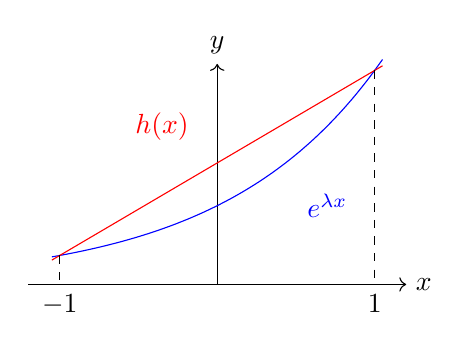
\begin{tikzpicture}
            \draw[->] (-2.4, 0) -- (2.4, 0) node[right] {$x$};
            \draw[->] (0, 0) -- (0, 2.8) node[above] {$y$};
            \draw[scale=1, domain=-2.1:2.1, smooth, variable=\x, blue] plot ({\x}, {e^(\x/2)});
            \draw[scale=1, domain=-2.1:2.1, smooth, variable=\y, red]  plot ({\y}, {(e+1/e)/2 + (e-1/e) * \y/4}); % Divided \x and \y by 2 on the 2nd coordinate to scale the y axis by 1/2.
                \node[text=red] at (-0.7,2) {$h(x)$};
            \node[text=blue] at (1.4,1) {$e^{\lambda x}$};
            \draw [dashed] (-2, {e^(-1)}) -- (-2,0)  node[below] {$-1$};
            \draw [dashed] (2, {e^(1)}) -- (2,0) node[below] {$1$};
        \end{tikzpicture} 
    \end{tabular}
    \end{tabular}

    As the picture above shows, $h(x)$ is the line that passes through the points $x = -1$ and $x = 1$ in the function $e^{\lambda x}$. Since $e^{\lambda x}$ is convex ($\lambda > 0$), it follows that $h(x) \geq e^{\lambda x} $ for $x \in [-1,1]$. Thus,

    \[\everymath{\displaystyle}\arraycolsep=1.8pt\def\arraystretch{1.8}
      \begin{array}{rcl}
        \E[e^{\lambda Y_i}] & \leq & \E[h(Y_i)] \\
        \text{\scriptsize ($h$ is linear)}& = & h(\E Y_i) = h(0)\\
        & = & \frac{e^\lambda + e^{-\lambda}}{2} = \cosh \lambda .
      \end{array}      
    \]
    Finally, $(2k)! \geq 2^k \cdot k! $, for every $k\in\N$. Thus,

    \[
        \E[e^{\lambda Y_i}]\leq \cosh \lambda \;=\; \sum_{k = 0}^\infty \frac{\lambda^{2k}}{(2k)!} \;\leq\; \sum_{k = 0}^\infty \frac{\lambda^{2k}}{2^k \cdot k!} \;=\; e^{\lambda^2 / 2}.
    \]

    \end{proof}

    Now, define $Y_i = X_i - X_{i-1}$. Then, by hypothesis, $|Y_i| \leq 1$ and
    \[ \E [Y_i | X_{i-1},\ldots, X_0] = \E [X_i - X_{i-1} | X_{i-1},\ldots, X_0] = X_i - X_i = 0. \] 
    Therefore, we can apply the previous inequality to assert,
    \[ \E [e^{\lambda Y_i} | X_{i-1},\ldots, X_0] \leq e^{\lambda^2/2}. \tag*{$ (\star) $}\]

    Using the formula $E[XY] = E_X [X E[Y|X]]$ we assert that
    \[ \E e^{\lambda X_m} \; = \;  \E\left[\prod_{i = 1}^{m-1} e^{\lambda Y_i} \cdot \E[e^{\lambda Y_m} | X_{m-1},\ldots, X_0]\right] \]

    We repeat this process $n$ times:
    \[ \everymath{\displaystyle}\arraycolsep=1.8pt\def\arraystretch{1.8}
        \begin{array}{r c c c l}
        & & \E e^{\lambda X_m}  =   \E \prod_{i = 1}^{m} e^{\lambda Y_i} \hfill\\
        & = & \E\left[\prod_{i = 1}^{m-1} e^{\lambda Y_i} \cdot \E[e^{\lambda Y_m} | X_{m-1},\ldots, X_0]\right] \hfill & \overset{(\star)}{\leq} & \E\left[\E \prod_{i = 1}^{m-1} e^{\lambda Y_i} \right] e^{\lambda^2 / 2}\\
        & = & \E\left[\prod_{i = 1}^{m-2} e^{\lambda Y_i} \cdot \E[e^{\lambda Y_{m-1}} | X_{m-2},\ldots, X_0]\right]e^{\lambda^2 / 2} & \overset{(\star)}{\leq} & \E\left[\E \prod_{i = 1}^{m-2} e^{\lambda Y_i} \right] e^{2\lambda^2 / 2}\\
        & = & \hfill\vdots\hfill & \leq & \hfill\vdots\hfill\\
        & = & \E\left[\E[e^{\lambda Y_{1}} |  X_0]\right]e^{\lambda^2 / 2} & \leq & \hfill e^{m\lambda^2/2} \hfill
    \end{array} \tag*{$ (*) $} \]
    At last, by setting $\lambda = t/\sqrt{m}$ we obtain,
    \[ \everymath{\displaystyle}\arraycolsep=1.8pt\def\arraystretch{1.8}
    \begin{array}{r c l}
        \P\{X_m > t\sqrt{m}\} & = & \P\{e^{\lambda X_m} > e^{\lambda t \sqrt{m}}\} \\
        \text{\scriptsize (Markov)}& \leq & \E[e^{\lambda X_m} ] e^{-\lambda t \sqrt{m}}\\
        & \overset{(*)}{\leq} & e^{m\lambda^2/2} \cdot e^{-\lambda t \sqrt{m}}\\
        \text{\scriptsize ($\lambda = t/\sqrt{m}$)} & = & e^{t^2/2} e^{-t^2} = e^{-t^2 / 2}.
    \end{array}    \tag*{$ (\bullet) $}
    \]
\end{proof}
%% --------------------

\begin{remark} We assumed that $X_0 = 0$ to lighten the notation. However, we can remove this restriction by replacing $X_m$ with $X_m - X_0$ in some crucial steps:
    \[\everymath{\displaystyle}\arraycolsep=1.8pt\def\arraystretch{1.8}
        \begin{array}{rl}
            & X_m-X_0 = \sum_{i = 1}^n Y_i\\
            \overset{(*)}{\implies} & \E e^{\lambda (X_m-X_0)} = \E \prod_{i = 1}^{m} e^{\lambda Y_i} \leq e^{m \lambda^2 / 2}\\
            \overset{(\bullet)}{\implies} & \P\{X_m-X_0 > t\sqrt{m}\} \leq e^{-t^2/2}
        \end{array} 
        \] 

\end{remark}    

In the following section we are going to present an application of the Azuma-Hoeffding inequality to prove the convergence to the mean of a fast (but not effective) approximation algorithm for the \textit{Travelling Salesman Problem}. 

\section{An Heuristic Algorithm for the Travelling Salesman Problem}

Let $X_1,\ldots, X_N$ be a sample of $N$ uniformly distributed points in a compact square $[0,L]\times [0,L]$. The algorithm divides this square in $M$ stripes of width $L/M$ each. Then, it connects each of the points in each of the stripes vertically and connects the top-most of one stripe with the top-most of the next one (or viceversa as the image below shows).

\begin{figure}[ht]\label{TSP:pic0}
    \centering
    \subfloat[Uniform sample]{\label{TSP:pic0.1}
        \includegraphics[width=0.33\textwidth]{../Simulation/TSPPictures/ex0.png}
    }
    \subfloat[Divide in $M$ stripes]{\label{TSP:pic0.2}
        \includegraphics[width=0.33\textwidth]{../Simulation/TSPPictures/ex1.png}
    }
    \subfloat[Join points vertically]{\label{TSP:pic0.3}
        \includegraphics[width=0.33\textwidth]{../Simulation/TSPPictures/ex2.png}
    }
\end{figure}

In the paper~\cite{gzyl1990physicist} the authors found that the optimal  number of stripes is $M^* = \floor{0.58 N^{1/2}}$. If $t_N$ is the TSP solution distance for our sample and $d_N$ is the algorithm's answer with the optimal $M^*$, then the error is asymptotically:
\[  \frac{d_N-t_N}{t_N} \approx 0.23.\] 

The result that we are going to show is that $d_n$ is very concentrated around its mean. In order to prove this, some modifications must be made to the algorithm's trajectory. Let $e_N$ be the distance of a new trajectory that satisfies the following conditions:
\begin{itemize}
    \item For any empty stripe in the plane we sum the length of its diagonal $\sqrt{L^2+ L^2/M^2}$ and then it skips the empty stripe.
    \item When there are no empty stripes, $e_N = d_N$ 
\end{itemize}
 Since the probability that any given stripe is empty converges exponentially to 0,
\[ \begin{array}{rl}
    {(1- 1/M)}^N & = {(1- 0.58^{-1} N^{-1/2})}^N\\[1em]
    & = {\left({(1- 1/M)}^{M}\right)}^{0.58^{-1} N^{1/2}}\\[1em]
    &  \sim \exp(-0.58^{-1} N^{1/2}).
\end{array} \] 


Let $\A_i := \sigma\{X_1,\ldots,X_i\}$ denote the sigma algebra corresponding to revealing the first $i$ points, $\A_0 = \{\emptyset, {[0,L]}^2\}$. The expected value of the trajectory $e_N$ given that we only know the positions of the first $i$ points in the sample is $\E (e_N | \A_i)$. Define
\[ Z_i = \E (e_N | \A_i) - \E (e_N | \A_{i-1}),  \]  
As the difference of this expectations when we reveal 1 more point. Note that since
\[ \E(Z_i | \A_i) =  \E (e_N | \A_i, \A_i) - \E (e_N | \A_{i-1}, A_i) = \E (e_N | \A_i) - \E (e_N | \A_i) = 0,\] 
$Z_1, \ldots, Z_N$ is the difference sequence of a vertex exposure martingale.

% \begin{figure}[ht]\label{TSP:pic1}
%     \subfloat[$i = 0$]{\label{TSP:pic1.1}
%         \includegraphics[width=0.25\textwidth]{../Simulation/TSPPictures/pic0.png}
%     }
%     \subfloat[$i = 1$]{\label{TSP:pic1.2}
%         \includegraphics[width=0.25\textwidth]{../Simulation/TSPPictures/pic1.png}
%     }
%     \subfloat[$i = 2$]{\label{TSP:pic1.3}
%         \includegraphics[width=0.25\textwidth]{../Simulation/TSPPictures/pic2.png}
%     }
%     \subfloat[$i = 4$]{\label{TSP:pic1.4}
%         \includegraphics[width=0.25\textwidth]{../Simulation/TSPPictures/pic3.png}
%     }

%     \subfloat[$i = 7$]{\label{TSP:pic1.5}
%         \includegraphics[width=0.25\textwidth]{../Simulation/TSPPictures/pic4.png}
%     }
%     \subfloat[$i = {12}$]{\label{TSP:pic1.6}
%         \includegraphics[width=0.25\textwidth]{../Simulation/TSPPictures/pic5.png}
%     }
%     \subfloat[$i = {18}$]{\label{TSP:pic1.7}
%         \includegraphics[width=0.25\textwidth]{../Simulation/TSPPictures/pic6.png}
%     }
%     \subfloat[$i = N = 50$]{\label{TSP:pic1.8}
%         \includegraphics[width=0.25\textwidth]{../Simulation/TSPPictures/ex2.png}
%     }
%     \caption{Evolution of the vertex exposure martingale}
% \end{figure}

Define $e_N^{[i]}$ as the distance of the trajectory when we remove the $i$-th point from the sample. Intuitively from the triangle inequality, we can obtain the following inequalities:
\[ e_N^{[i]} \leq e_N \leq e_N^{[i]} + 2 L/M, \]
meaning that revealing one point cannot increase more than 2 widths the distance of the trajectory. Thus,
\[ \|Z_i\|_\infty = \sup_{X_1,\ldots, X_N} \|\E (e_N | \A_i) - \E (e_N | \A_{i-1})\| \leq 2L/M. \tag*{$ (\star)$}.\]

On the other hand,
\[  e_N - \E e_N = \E (e_N | \A_N) - \E (e_N | \A_{0}) = \sum_{i = 1}^{N} Z_i.\]
Therefore, by the Azuma-Hoeffding inequality,
\[ \P \{ |e_N - \E e_N| > t \} \leq 2\exp\left(\frac{-t^2}{2}\sum_{i = 1}^{N} \|Z_i\|_{\infty}^2 \right). \] 
Finally,
\[ \sum_{i = 1}^{N} \|Z_i\|_{\infty}^2 \leq \frac{4NL^2}{M^2}, \]
which implies that
\[\P \{ |e_N - \E e_N| > t \} \leq 2\exp\left(\frac{-t^2}{2}\sum_{i = 1}^{N} \frac{4NL^2}{M^2} \right) \sim e^{-t^{2} K N}, \] 
for some $K\in \R^+$.

\section{Lipschitz Condition and Three Additional Examples}

Three examples from~\cite{alon2016probabilistic} will be exposed to illustrate some ideas that can be associated with the main inequality of this chapter. Furthermore, the usefulness of the Azuma-Hoeffding inequality in the study of graphs and metric spaces can be used in a more general frame by defining the Lipschitz condition.

\vspace*{1em}

Let $\Omega = A^B$ be the set of all functions $g: B\to A$ for which a probability measure is assigned
\[ \P\{g(b) = a\} = p(a,b),\hspace*{1em} \sum_{a\in A} p(a,b) = 1. \]
All the values $g(b)$ are mutually independent. Now, fix a chain of sets 
\[ \emptyset = B_0 \subset B_1 \subset \ldots \subset B_m = B,\hspace*{1em} \mathcal{B} = {\{B_i\}}_{i = 0}^m \]
and let $L: A^B \to \R$ be a functional. The martingale sequence $X_0,\ldots, X_m$ associated with $L$ and $\mathcal{B}$ is defined as it follows: For a fixed $h \in A^B$:

\[ X_i(h) = \E[ L(g) \;|\; g(b) = h(b),\; \forall b\in B_i ]. \] 

What this means is that, given that we know the values in $B_i$ of a function $h$, the martingale at the $i$-th step predicts the outcome of $L(h)$ based only on this information. The following definition and theorem have the purpose to make our lives easier when talking about the `boundness' of a martingale.

\begin{definition}
    A functional $L$ is said to satisfy the Lipschitz condition if for every $i < m$: Whenever two functions $g, g'$ differ only in $B_{i+1}- B_i$,
    \[ |L(g) - L(g')| \leq 1. \] 
\end{definition}

When we say that the outcome of $L$ won't change by more than 1 unit from one revelation to another, it means that it has the Lipschitz condition. The following theorem will connect this idea to Azuma's inequality:

\begin{theorem}\label{lipschitz-condition}
    The martingale associated with a functional $L$ with the Lipschitz condition satisfies:
    \[ |X_{i+1}(g)- X_i(g)| \leq 1,\hspace*{1em} \forall g\in A^B,\; \forall i < m. \] 
\end{theorem}

\begin{proof} The proof is adapted from~\cite{alon2016probabilistic} chapter 7. In the original proof, the author skips many steps that I believe are not trivial. Thus, I decided to restructure the proof using the same notation they used in the source material:

\subsubsection*{Preliminaries}
Our goal is to calculate $|X_{i+1}(h) - X_{i}(h)|$, so fix $h \in A^B$, $i\in \N$ and define

\[ p_{f}^{(j)} = \P\{g = f \;|\; g(b) = h(b),\; \forall b \in B_{j}\}.\; \forall j\in \N. \]

Now, $\forall j\in \N$, define $H^{(j)}\subset A^B$ to be the set of functions $f$ in which $h(b) = f(b)$ for every $b \in B_{j}$. In notation,

\[ H^{(j)} = \{f \in A^B: h(b) = f(b),\; \forall b \in B_j\}. \] 

Note that if $h' \not\in H^{(j)}$ and $g(b) = h(b)$ for every $b\in B_{j}$, then it would be imposible for $g$ to be equal to $h'$ because there would exist $b^* \in B_{j}$ such that $h'(b^*) \neq h(b^*) = g(b^*)$. Thus, if $h' \not\in H^{(j)}$, then $p_{h'}^{(j)} = 0$. This also implies that 
\[\sum_{h' \in H^{(j)}} p_{h'}^{(j)} = 1 \] 

\subsubsection*{Rewriting $X_{i+1}$}
From now on, $H$ without any index refers to $H^{(i+1)} =: H$
\[\everymath{\displaystyle}\arraycolsep=1.4pt\def\arraystretch{1.5}
    \begin{array}{rcl}
    X_{i+1}(h) & = & \E[ L(g) \;|\; g(b) = h(b),\; \forall b\in B_{i+1} ]. \\ 
    & = & \sum_{h' \in A^B} L(h') \cdot \P\{g = h' \;|\; g(b) = h(b),\; \forall b \in B_{i+1}\}\\
    & = & \sum_{h' \in H} L(h') \cdot p_{h'}^{(i+1)}
\end{array}\]


\subsubsection*{Rewriting $X_i$}
Like the previous step,
\[\everymath{\displaystyle}\arraycolsep=1.4pt\def\arraystretch{1.5}
    \begin{array}{rcl}
    X_{i}(h) & = & \sum_{f\in H^{(i)}} L(f) p_{f}^{(i)}
\end{array}\]
However, we want to write the sum of $X_{i}(h)$ in terms of $h' \in H$. Now, for $h' \in H$, let $H[h']$ be the set of $h^*$ such that $h^*, h'$ that can only differ in $B_{i+1}-B_{i}$. In notation,
\[ H[h'] = \left\{ h^*: \begin{matrix}
    h^*(b) = h'(b),\; \forall b\in B-B_{i+1}\\
    h^*(b) = h'(b) ,\; \forall b\in B_{i}
\end{matrix} \right\} \] 
Also, define for $h^* \in H[h']$
\[ q_{h^*} = \P\{g(b) = h^*(b),\; \forall b\in B_{i+1} \;|\; g(b) = h(b),\; \forall b\in B_{i} \}. \]
It follows from the definition of $H[h']$ and $H$ that
\[ \everymath{\displaystyle}\arraycolsep=1.4pt\def\arraystretch{1.5}
    \begin{array}{rcl}
    \sum_{h^* \in H[h']} q_{h^*} & = & \sum_{h^* \in H[h']} \P\left\{\begin{matrix} g(b) = h^*(b),\; \forall b\in B_{i+1}-B_i\\  g(b) = h^*(b) = h'(b) ,\; \forall b\in B_i \end{matrix} \;\Bigg|\; g(b) = h(b) = h'(b),\; \forall b\in B_{i} \right\} \\
     & = & \P\{g(b) = h'(b),\; \forall b\in B_{i} \;|\; g(b) = h'(b),\; \forall b\in B_{i} \}\\
     & = & 1.
\end{array} \]  

$\coprod$ is the notation I'm going to use for the disjoint union. Note that if $h_1'\neq h_2' \in H$, then both must differ in some $b \in B- B_{i+1}$. Thus, the following unions are disjoint
\[\everymath{\displaystyle}\arraycolsep=1.4pt\def\arraystretch{1.5}
    \begin{array}{rcl}
    \coprod_{h' \in H} H[h'] & = & 
    \coprod_{h' \in H} \left\{ h^*: \begin{matrix}
        h^*(b) = h'(b),\; \forall b\in B-B_{i+1}\\
        h^*(b) = h'(b) = h(b) ,\; \forall b\in B_{i}
    \end{matrix} \right\}\\
   \hfill\vdots\hfill & = & \coprod_{h' \in H} \left\{ h^*: \begin{matrix}
        h^*(b) = h'(b),\; \forall b\in B-B_{i+1}\\
        h^*(b) = h(b) ,\; \forall b\in B_{i}
    \end{matrix} \right\}\\
    \hfill\downarrow\hfill& = & \{h^*: h^*(b) = h(b) ,\; \forall b\in B_{i} \}\\
    \coprod_{h' \in H} \coprod_{h^* \in H[h']}\{h^*\} & = & H^{(i)}.
\end{array} \] 
Thus, we can make a partition of $X_i(h)$ iterating over $H$ and $H[h']$:
\[\everymath{\displaystyle}\arraycolsep=1.4pt\def\arraystretch{1.5} 
\begin{array}{lcl}
    \E[L(g) \;|\; g(b) = h(b),\; \forall b\in B_{i}] & = & \sum_{f\in H^{(i)}} L(f) p_{f}^{(i)}\\
    & = &  \sum_{h' \in H}\sum_{h^* \in H[h']} L(h^*) p^{(i)}_{h^*}
\end{array}\] 

Finally, for $h' \in H$ and $h^* \in H[h']$,
\[ \everymath{\displaystyle}\arraycolsep=1.4pt\def\arraystretch{1.5} 
\begin{array}{lll}
    & & p^{(i)}_{h^*} = \\
    & & \P\{g = h^* \;|\; g(b) = h(b),\; \forall b\in B_i\}\\
    & = & \P\{g = h^* | g(b) = h^*(b),\; \forall b\in B_{i+1} \} \cdot \P\{g(b) = h^*(b),\;\forall b\in B_{i+1} | g(b) = h^*(b),\; \forall b\in B_{i} \}\\
    & = & \P\{g = h' | g(b) = h(b),\; \forall b\in B_{i+1} \} \cdot q_{h^*}\\
    & = & p_{h'}^{(i+1)}\cdot q_{h^*}
\end{array}  \] 
\[ \implies X_i(h) = \sum_{h' \in H}\sum_{h^* \in H[h']} [L(h^*) q_{h^*}] \cdot p_{h'}^{(i+1)} \] 

\subsubsection*{Bound for $|X_{i+1}- X_i|$}
Combine the results from the two previous sections. For the second line, remember that $\sum_{h^*\in H[h']} q_{h^*} = 1$
\[ \everymath{\displaystyle}\arraycolsep=1.4pt\def\arraystretch{2.9} 
\begin{array}{rcl}
    |X_{i+1}(h)- X_i(h)| & = & \left|\sum_{h' \in H}p_{h'}^{(i+1)} \left[ L(h') - \sum_{h^* \in H[h']}  L(h^*)q_{h^*}\right] \right|\\
    & = & \left|\sum_{h' \in H}p_{h'}^{(i+1)} \sum_{h^* \in H[h']} q_{h^*}(L(h') - L(h^*)) \right|\\
    & \leq & \sum_{h' \in H}p_{h'}^{(i+1)} \sum_{h^* \in H[h']} q_{h^*} |L(h') - L(h^*)|
\end{array} \] 

By hypothesis, $|L(h') - L(h^*)| \leq 1$. Thus,

\[|X_{i+1}(h)- X_i(h)| \leq  \sum_{h' \in H}p_{h'}^{(i+1)} \sum_{h^* \in H[h']} q_{h^*} = \sum_{h' \in H}p_{h'}^{(i+1)} = 1. \] 

\end{proof}

With this theorem, we can talk with more freedom about the boundness of a martingale. The following three examples will illustrate some uses for Azuma's inequality in conjunction with the previous theorem.

\subsection*{Example 1}
Let $g \in {[n]}^{n}$ be a random vector (uniformly chosen) with $n$ entries, in which every entry is in $[n] = \{1,\ldots n\}$. Define $L(g)$ to be the amount of number that are not included in the vector,
\[ L(g) = \# \{ k \;:\; g_i \neq k,\; \forall i \in [n]\} = \sum_{k = 1}^{n} \1_{k \not\in g} \] 
For example,

\[ L(\underset{g_1}{1},\underset{g_2}{3},\underset{g_3}{1},\underset{g_4}{6},\underset{g_5}{4},\underset{g_6}{3}) = 2.\;\text{ (because 2 and 5 are missing)} \]

We can understand the process of choosing $g$ as independently assigning a random number in each of its coordinates. Thus, for a number $k \in \{1,\ldots, n\}$, the probability that this number is not in any of the entries of the vector is
\[\E \1_{k \not\in g} = \P\{g_i \neq k, \; \forall i\} = \prod_{i = 1}^n P\{g_i \neq k\} = {\left(1-\tfrac{1}{n}\right)}^n. \] 
Hence,
\[ \E L(g) = \sum_{k = 1}^n \P\{g_i \neq k, \; \forall i\} = n {\left(1-\tfrac{1}{n}\right)}^n \sim \frac{n}{e}. \] 
Now, define $B_i = \{1, \ldots, i\}$
\[\begin{array}{rcl}
    X_0(h) & = & \E L(g) \sim \frac{n}{e},\\
    X_1(h) & = & \E [ L(g) \;|\; g_1 = h_1 ], \\
    \hfill\vdots\hfill & = & \vdots \\
    X_j(h) & = & \E [L(g) \;|\; g_i = h_i,\; \forall i\leq j ],\\
    \hfill\vdots\hfill & = & \vdots \\
    X_n(h) & = & \E [L(g) \;|\; g_i = h_i,\; \forall i\leq n] = L(h).
\end{array} \] 
The value of $L(g)$ can vary at most by 1 for each coordinate we reveal, so $L(g)$ has the Lipschitz condition. Then, we use \text{theorem}~\ref{lipschitz-condition} and Azuma-Hoeffding inequality to conclude that
\[ \P\{|L(g) - \tfrac{n}{e}| > t\sqrt{n}\} < 2e^{-t^2 / 2}. \] 

\subsection*{Example 2}
Here's a case where using {theorem}~\ref{lipschitz-condition} will give us worse results. Let $\sigma_1,\ldots, \sigma_n$ be Rademacher random variables, and $v_1,\ldots, v_n$ fixed vectors in the closed unit ball. Define

\[ X = \left| \sum_{i = 1}^n \sigma_i v_i \right|.\]

The goal here is to find an exponential bound for the tail distribution of $X$. We create a martingale that exposes the value of $\sigma_i$ one $i$ at a time. Let $\sigma' = (\sigma_1',\ldots, \sigma_n') \in {\{-1,1\}}^n$,

\[\begin{array}{rcl}
    X_0(\sigma') & = & \E |\sum_{i = 1}^n \sigma_i v_i|\\
    X_1(\sigma') & = & \E [ |\sum_{i = 1}^n \sigma_i v_i| \;|\; \sigma_1 = \sigma_1' ] \\
    \hfill\vdots\hfill & = & \vdots \\
    X_j(\sigma') & = & \E [|\sum_{i = 1}^n \sigma_i v_i| \;|\; \sigma_i = \sigma_i',\; \forall i\leq j ]\\
    \hfill\vdots\hfill & = & \vdots \\
    X_n(\sigma') & = & \E [|\sum_{i = 1}^n \sigma_i v_i| \;|\; \sigma_i = \sigma_i',\; \forall i\leq n] = X.
\end{array} \]

The value on one coordinate can alter $X$ to a maximum of 2 units. Thus, we could apply {theorem}~\ref{lipschitz-condition} to conclude that $|X_{i+1}- X_i| \leq 2$. However, note that if $\sigma'$, $\sigma^*$ are two $n$-tuple that only differ on one coordinate, it follows from linearity of expectation that
\[ X_i(\sigma') = \frac{1}{2}(X_{i+1}(\sigma^*)+ X_{i+1}(\sigma')) \]
\[ \implies X_i(\sigma') - X_{i+1}(\sigma')  = \frac{1}{2}(X_{i+1}(\sigma^*)- X_{i+1}(\sigma'))\] 
\[ \implies  |X_i(\sigma') - X_{i+1}(\sigma')|  = \frac{1}{2}|X_{i+1}(\sigma^*)- X_{i+1}(\sigma')| \leq 1.\]
Thus, we can apply now Azuma's inequality and conclude the following
\[ \P\{X - E X > t \sqrt{n}\} < e^{-t^2/2}, \] 
\[ \P\{X - E X < -t \sqrt{n}\} < e^{-t^2/2}. \]
\subsection*{Example 3}
Let $\rho$ denote the Hamming metric in the space ${\{0,1\}}^n$, that is
\[ \rho(x,y) = \#\{i : x_i \neq y_i\}. \]
Let $B(A,s)$ be the set $\{y \;:\; \exists x\in A,\;\rho(x)\leq s\}$. The following theorem holds,

\begin{theorem} Let $\varepsilon, t > 0$ satisfy $\varepsilon = e^{-t^2 / 2}$. Then,
    \[ |A| \geq \varepsilon 2^n \implies |B(A,2t\sqrt{n})| \geq (1-\varepsilon) 2^n. \] 
\end{theorem}

\vspace*{1em}

\textit{Solution:} Assign a probability space to ${\{0,1\}}^n$ where all the points have the same probability of being chosen at random. Let $X(y) = \min_{x\in A} \rho(x,y)$, then create a martingale $X_0, \ldots, X_n$ based on the number of coordinates of $\{0,1\}^n$ exposed, that is,
\[ X_j(y) = \E [\min_{x\in A} \rho(x,z) \; | \; z_i = y_i,\; \forall i\leq j]. \]
In this case, note that if $y, y'$ differ in just one coordinate, then
\[ |X(y) - X(y')| \leq 1. \]
So we can use Azuma's inequality to conclude that
\[ \P\{X < \E X - t\sqrt{n}\} < e^{-\lambda^2/2} = \varepsilon \]   
\[ \P\{X > \E X + t\sqrt{n}\} < e^{-\lambda^2/2} = \varepsilon. \]   

Finally, since $P\{X = 0\} = |A|2^{-n} \geq \varepsilon$, it follows that $\E X \leq t\sqrt{n}$. Therefore,
\[ \P\{X > 2t\sqrt{n}\} < \varepsilon, \]
and as a consequence,
\[ |B(A,2t\sqrt{n})| = 2^n\P\{X > 2t\sqrt{n}\} \geq 2^n (1-\varepsilon) .  \] 

\vspace*{3em}


\backmatter{}

% The bibliography will go here
\end{document}
